% P18 project report in the Natural Language Engineering (NLE) template
% (nle.cls, Cambridge University Press), as required for NLP projects.

\documentclass{nle}

\usepackage{graphicx}
\usepackage{amsmath}
\usepackage{amssymb}
\usepackage{url}

\title[PEFT Showdown: Full FT vs LoRA vs Adapters vs Prompt Tuning]
      {Parameter-Efficient Fine-Tuning Showdown:\\
       Full Fine-Tuning vs LoRA vs Adapters vs Prompt Tuning}
\author[D. Mandal and others]
       {D\ls E\ls E\ls P\ls A\ls K\ns M\ls A\ls N\ls D\ls A\ls L,\ns
        A\ls N\ls O\ls O\ls P\ns K\ls U\ls M\ls A\ls R,\\
        C\ls H\ls I\ls R\ls A\ls N\ls J\ls E\ls E\ls T\ns B\ls I\ls S\ls W\ls A\ls S\\
        and\ns B\ls Y\ls A\ls G\ls A\ls R\ls I\ns P\ls R\ls A\ls V\ls E\ls E\ls N\ns K\ls U\ls M\ls A\ls R\\
        Team 18 (P18), Deep Learning Project, Sitare University\\
        \texttt{\{su-24039, su-24017, su-24037, su-24034\}@sitare.org}}

\received{November 2026}

\pagerange{\pageref{firstpage}--\pageref{lastpage}}
\pubyear{2026}

\begin{document}

\label{firstpage}
\maketitle

\begin{abstract}
We compare four ways of adapting \texttt{roberta-base} to a text classification task: full fine-tuning (Full FT), LoRA, bottleneck adapters and prompt tuning. Every method uses the same data splits, seeds, sequence length, batch size, epochs and GPU type. We report accuracy (and F1 on MRPC), trainable parameters, peak GPU memory, training time and checkpoint size on GLUE SST-2, MRPC and RTE, with the full training set and with only 1,000 training examples. The study has 122 training runs: 64 for the main grid, 16 for a learning-rate search and 42 for ablations. Adapters are tied with Full FT on accuracy while training 1.9\% of the parameters and using 42\% less peak GPU memory. LoRA is 0.3--2.1 points behind Full FT with 0.71\% of the parameters and a 3.4\,MB checkpoint. With 1,000 examples, Full FT and adapters lose the least accuracy. At this model size, prompt tuning stays close to the majority-class baseline on MRPC and RTE, as Lester {\it et al.} \shortcite{lester2021} predict.
\end{abstract}

\section{Introduction}

Full fine-tuning updates every weight of a pretrained model. For each new task this means storing another full copy of the model (about 500\,MB for \texttt{roberta-base}) and keeping optimizer state for all 125M parameters in GPU memory. Parameter-efficient fine-tuning (PEFT) methods freeze the pretrained weights and train only a small number of new or selected parameters.

Published comparisons often differ in base model, training budget, or how trainable parameters are counted (for example, whether the classification head is included). We compare full fine-tuning, LoRA \cite{hu2022}, adapters \cite{houlsby2019} and prompt tuning \cite{lester2021} under one fixed setup on three GLUE tasks \cite{wang2019}. We answer four questions:
\begin{enumerate}
  \item How close does each PEFT method get to Full FT, and at what parameter cost?
  \item Which method loses the least accuracy when only 1,000 training examples are available?
  \item Why is prompt tuning weak at this model size?
  \item Which method should be used under a memory limit, a time limit, or with very little data?
\end{enumerate}
Code and all result files are available at\\ \url{https://github.com/Anoop1230-tech/peft-showdown}.

\section{Background}

\paragraph{Adapters.} Houlsby {\it et al.} \shortcite{houlsby2019} insert small bottleneck MLPs into every transformer layer: a down-projection to dimension $m$, a nonlinearity, an up-projection back to the hidden size $d$, and a residual connection. The Houlsby variant places one adapter after the attention block and one after the feed-forward block. Pfeiffer {\it et al.} \shortcite{pfeiffer2021} use a single adapter after the feed-forward block. Houlsby {\it et al.} reach within 0.4\% of full fine-tuning on GLUE while training about 3.6\% of the parameters per task.

\paragraph{LoRA.} For a frozen weight matrix $W_0 \in \mathbb{R}^{d\times k}$, LoRA \cite{hu2022} learns a low-rank update, so the layer computes
\[ h = W_0x + \frac{\alpha}{r}BAx, \qquad B \in \mathbb{R}^{d\times r},\; A \in \mathbb{R}^{r\times k}, \]
with a small rank $r$. $B$ starts at zero, so training starts from the pretrained model. After training, $BA$ can be merged into $W_0$, so inference costs nothing extra.

\paragraph{Prompt tuning.} Lester {\it et al.} \shortcite{lester2021} freeze the model and prepend $p$ learnable ``virtual token'' embeddings to the input. Only these embeddings are trained. With T5 they show that the gap to full fine-tuning is large for small models and closes only at around 10B parameters.

\section{Methods}

All methods use \texttt{roberta-base} \cite{liu2019} (12 layers, hidden size 768) with RoBERTa's classification head (a $768{\times}768$ dense layer with tanh and a $768{\times}2$ projection, 592,130 parameters). The head is trained in every method and counted in every trainable-parameter number. Table~\ref{tab:methods} lists the method settings. LoRA and prompt tuning use the Hugging Face \texttt{peft} library (0.21.2). \texttt{peft} has no Houlsby adapters, so adapters use the AdapterHub \texttt{adapters} library (1.3.0), which is built on the same \texttt{transformers} models.

\begin{table}
  \caption{Methods, trainable parameters (classification head included) and learning rates}
  \label{tab:methods}
  \begin{minipage}{\textwidth}
    \begin{tabular}{llrrl}
    \hline\hline
    Method & Settings & Trainable & \% & LR \\
    \hline
    Full FT & all weights & 124,647,170 & 100.00 & 2e-5 \\
    LoRA & $r{=}8$, $\alpha{=}16$, query/value & 887,042 & 0.71 & 5e-4 \\
    Adapters & Houlsby, rf 16 ($m{=}48$) & 2,381,186 & 1.87 & 3e-4 \\
    Prompt tuning & 20 virtual tokens, random init & 607,490 & 0.48 & 1e-2 \\
    \hline\hline
    \end{tabular}
  \end{minipage}
\end{table}

\section{Experimental setup}

\paragraph{Same budget.} AdamW, weight decay 0.01, linear warmup over 6\% of the steps, batch size 32, maximum sequence length 128, fp16. Epochs: 3 for SST-2 full data, 10 for MRPC and RTE full data, 20 for every 1k run. Only the method-specific settings and the learning rate differ.

\paragraph{Splits.} GLUE test labels are hidden, so we report on the official validation split. We hold out 10\% of the training set as our dev split. The checkpoint with the best dev accuracy (evaluated every epoch) is kept, and the LR search also uses the dev split. The validation split is never used for any choice.

\paragraph{Low-data regime.} 1,000 examples are drawn from the training part with the run's seed, so every method sees the same examples for a given seed.

\paragraph{Seeds and measurements.} Seeds 1, 2 and 3 for every configuration, except SST-2 full data (seed 1 only, about one hour per Full FT run). We record trainable parameters (\texttt{requires\_grad}, head included), peak GPU memory (\texttt{torch.cuda.max\_memory\_allocated} after resetting the peak counter), wall-clock training time, and the size of the saved trainable weights. Each run is a separate process on one Tesla T4 (16\,GB) on Kaggle, and writes one validated JSON result file.

\paragraph{Learning-rate search.} Following our plan, we tried three learning rates per method with seed 1 on RTE and MRPC full data. For every method, the learning rate used in the final runs had the best mean dev accuracy (Table~\ref{tab:lr}), so the final runs did not need to be repeated.

\begin{table}
  \caption{LR search: dev accuracy ($\times$100), seed 1, full data. * = LR used in all final runs}
  \label{tab:lr}
  \begin{minipage}{\textwidth}
    \begin{tabular}{llrrr}
    \hline\hline
    Method & LR & RTE dev & MRPC dev & Mean \\
    \hline
    Full FT & 1e-5 & 76.7 & {\bf 88.3} & 82.5 \\
     & 2e-5* & {\bf 78.3} & 87.2 & {\bf 82.8} \\
     & 3e-5 & {\bf 78.3} & 86.9 & 82.6 \\
    \hline
    LoRA & 1e-4 & 70.7 & 86.9 & 78.8 \\
     & 3e-4 & 74.7 & {\bf 88.6} & 81.7 \\
     & 5e-4* & {\bf 75.9} & 88.3 & {\bf 82.1} \\
    \hline
    Adapters & 1e-4 & 71.1 & 86.9 & 79.0 \\
     & 3e-4* & {\bf 77.9} & 87.5 & {\bf 82.7} \\
     & 1e-3 & 75.9 & {\bf 88.0} & 82.0 \\
    \hline
    Prompt tuning & 1e-3 & 52.2 & 69.2 & 60.7 \\
     & 1e-2* & {\bf 55.8} & 72.8 & {\bf 64.3} \\
     & 3e-2 & 52.2 & {\bf 73.8} & 63.0 \\
    \hline\hline
    \end{tabular}
  \end{minipage}
\end{table}

\section{Results}

\subsection{Unified comparison}

Table~\ref{tab:main} gives the scores and Table~\ref{tab:eff} the efficiency numbers. Figure~\ref{fig:params} plots accuracy against trainable parameters.

\begin{table}
  \caption{GLUE validation accuracy (and F1 on MRPC) $\times$100, mean $\pm$ std over seeds 1--3 (SST-2 full: seed 1 only)}
  \label{tab:main}
  \begin{minipage}{\textwidth}
    \begin{tabular}{lccccc}
    \hline\hline
    Method & Data & SST-2 & MRPC acc & MRPC F1 & RTE \\
    \hline
    Full FT & full & 94.0 & 87.7 $\pm$ 1.4 & 91.2 $\pm$ 1.2 & 76.1 $\pm$ 2.2 \\
    LoRA & full & 93.7 & 87.1 $\pm$ 1.0 & 90.9 $\pm$ 0.6 & 74.0 $\pm$ 2.0 \\
    Adapters & full & 94.2 & 87.3 $\pm$ 0.6 & 91.0 $\pm$ 0.4 & 76.3 $\pm$ 1.8 \\
    Prompt tuning & full & 91.2 & 70.7 $\pm$ 1.9 & 81.5 $\pm$ 0.7 & 56.1 $\pm$ 2.6 \\
    \hline
    Full FT & 1k & 90.4 $\pm$ 0.5 & 85.8 $\pm$ 2.2 & 89.9 $\pm$ 1.4 & 69.9 $\pm$ 2.1 \\
    LoRA & 1k & 90.1 $\pm$ 0.5 & 84.3 $\pm$ 1.3 & 88.8 $\pm$ 0.9 & 66.9 $\pm$ 3.2 \\
    Adapters & 1k & 90.4 $\pm$ 0.8 & 84.4 $\pm$ 1.0 & 89.1 $\pm$ 0.8 & 71.2 $\pm$ 2.0 \\
    Prompt tuning & 1k & 73.7 $\pm$ 15.4 & 71.1 $\pm$ 2.5 & 81.9 $\pm$ 1.0 & 52.8 $\pm$ 2.7 \\
    \hline
    {\it Majority class} & & {\it 50.9} & {\it 68.4} & {\it 81.2} & {\it 52.7} \\
    \hline\hline
    \end{tabular}
  \end{minipage}
\end{table}

\begin{table}
  \caption{Efficiency. Peak memory is the maximum over a method's runs; times are on a Tesla T4 with full training data}
  \label{tab:eff}
  \begin{minipage}{\textwidth}\footnotesize
    \begin{tabular}{lrrrrrr}
    \hline\hline
    Method & Trainable & \% & Mem & RTE & SST-2 & Ckpt \\
     & params & & (MiB) & time (s) & time (s) & (MB) \\
    \hline
    Full FT & 124,647,170 & 100.00 & 3,264 & 158 & 492 & 475.5 \\
    LoRA & 887,042 & 0.71 & 1,937 & 112 & 324 & 3.4 \\
    Adapters & 2,381,186 & 1.87 & 1,884 & 106 & 378 & 9.1 \\
    Prompt tuning & 607,490 & 0.48 & 1,923 & 117 & 385 & 2.3 \\
    \hline\hline
    \end{tabular}
  \end{minipage}
\end{table}

\paragraph{Adapters} are within $\pm$0.4 points of Full FT on every full-data score (94.2 vs 94.0 on SST-2, 87.3 vs 87.7 on MRPC, 76.3 vs 76.1 on RTE). All of these gaps are smaller than one standard deviation (1.4--2.2 points on MRPC and RTE), so the two methods are tied on accuracy. Adapters train 1.9\% of the parameters, use 42\% less peak memory (1,884 vs 3,264\,MiB) and train 33\% faster on RTE (106 vs 158\,s).

\paragraph{LoRA} is 0.3 points behind Full FT on SST-2, 0.6 on MRPC and 2.1 on RTE. It trains fewer parameters than adapters (0.89M vs 2.38M), has a smaller checkpoint (3.4 vs 9.1\,MB) and is the fastest method on SST-2 (324 vs 492\,s).

\paragraph{Prompt tuning} is far behind on the two small tasks. On MRPC, 70.7\% accuracy and 81.5 F1 are almost the same as always predicting ``paraphrase'' (68.4\% and 81.2). On RTE, 56.1\% is 3.4 points above the majority class. With the 67k SST-2 examples it reaches 91.2\%, so it does learn when it gets enough data.

\paragraph{Memory and time} (Figures~\ref{fig:mem} and~\ref{fig:time}). All PEFT methods use about 40\% less peak memory than Full FT, because the optimizer only keeps state for the trainable parameters. They differ little from each other (1,884--1,937\,MiB), because the activations of the frozen backbone dominate. Prompt tuning makes every input 20 tokens longer, so it is not faster than LoRA or adapters despite training the fewest parameters.

\begin{figure}
  \centering
  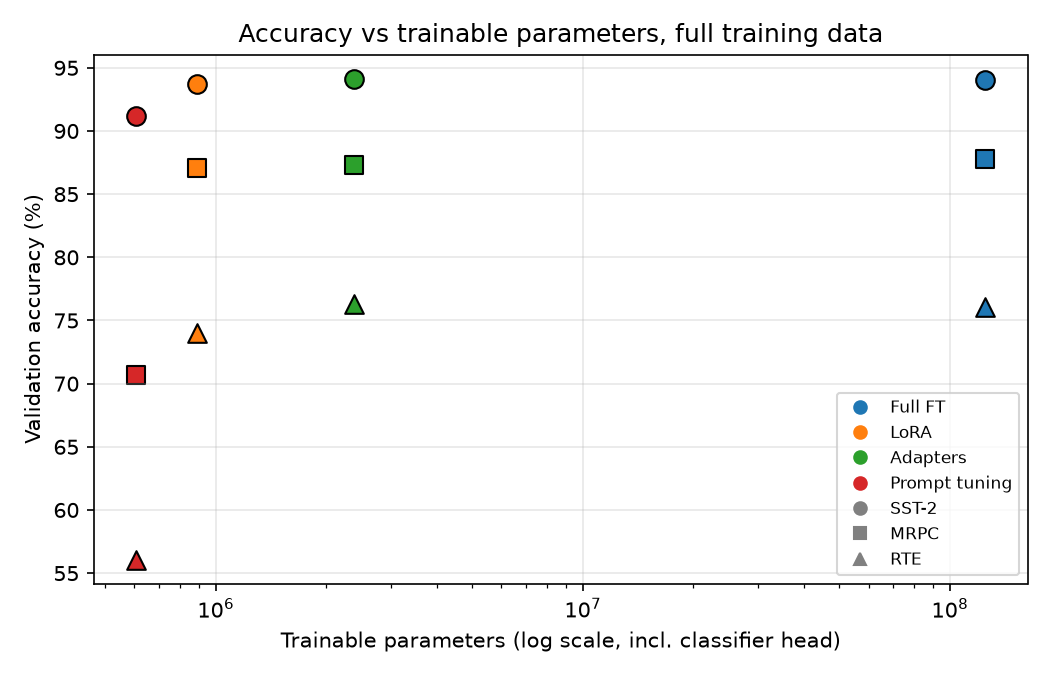
\includegraphics[width=0.8\textwidth]{figures/acc_vs_params.png}
  \caption{Validation accuracy vs trainable parameters (log scale), one point per method and task, full training data.}
  \label{fig:params}
\end{figure}

\begin{figure}
  \centering
  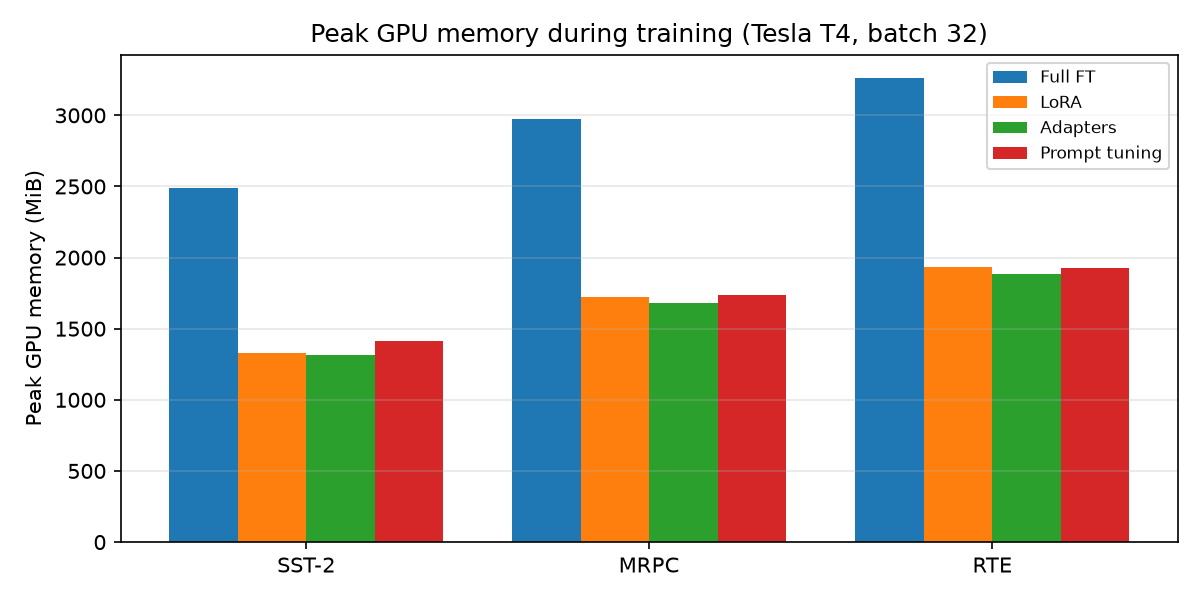
\includegraphics[width=0.7\textwidth]{figures/peak_memory.png}
  \caption{Peak GPU memory during training per method and task (Tesla T4, batch size 32).}
  \label{fig:mem}
\end{figure}

\begin{figure}
  \centering
  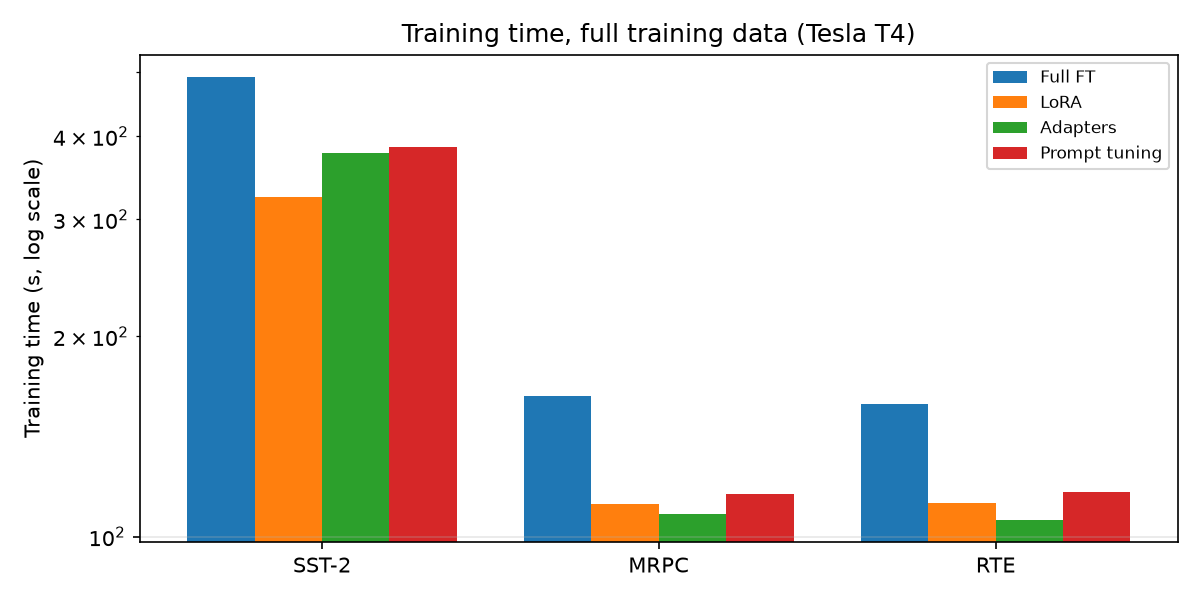
\includegraphics[width=0.7\textwidth]{figures/train_time.png}
  \caption{Training time per method and task, full training data (Tesla T4, log scale).}
  \label{fig:time}
\end{figure}

\subsection{Low-data regime}

Table~\ref{tab:lowdata} and Figure~\ref{fig:lowdata} show what happens with only 1,000 training examples. Full FT and adapters lose the least, 3.9 points on average. Adapters have the best RTE 1k score (71.2 vs 69.9 for Full FT), but their standard deviations (2.0 and 2.1) overlap, so we do not claim a clear winner. LoRA loses a bit more, mostly on RTE ($-$7.1, $\pm$3.2 across seeds).

Prompt tuning becomes unstable. On SST-2 1k, seeds 1 and 3 reach 83.7\% and 81.3\%, but seed 2 stays at 56.0\%, hence the $\pm$15.4 standard deviation. The best checkpoints of the working seeds were at epochs 17 and 20 of 20, so prompt tuning was still improving when training stopped. Its small drops on MRPC and RTE do not mean it holds up well: it was already near the majority-class baseline with full data.

\begin{table}
  \caption{Accuracy change (points) from full data to 1,000 training examples, mean over seeds}
  \label{tab:lowdata}
  \begin{minipage}{\textwidth}
    \begin{tabular}{lrrrr}
    \hline\hline
    Method & SST-2 & MRPC & RTE & Mean drop \\
    \hline
    Full FT & $-$3.7 & $-$2.0 & $-$6.1 & 3.9 \\
    LoRA & $-$3.6 & $-$2.8 & $-$7.1 & 4.5 \\
    Adapters & $-$3.8 & $-$2.9 & $-$5.1 & 3.9 \\
    Prompt tuning & $-$17.5 & +0.4 & $-$3.2 & 6.8 \\
    \hline\hline
    \end{tabular}
  \end{minipage}
\end{table}

\begin{figure}
  \centering
  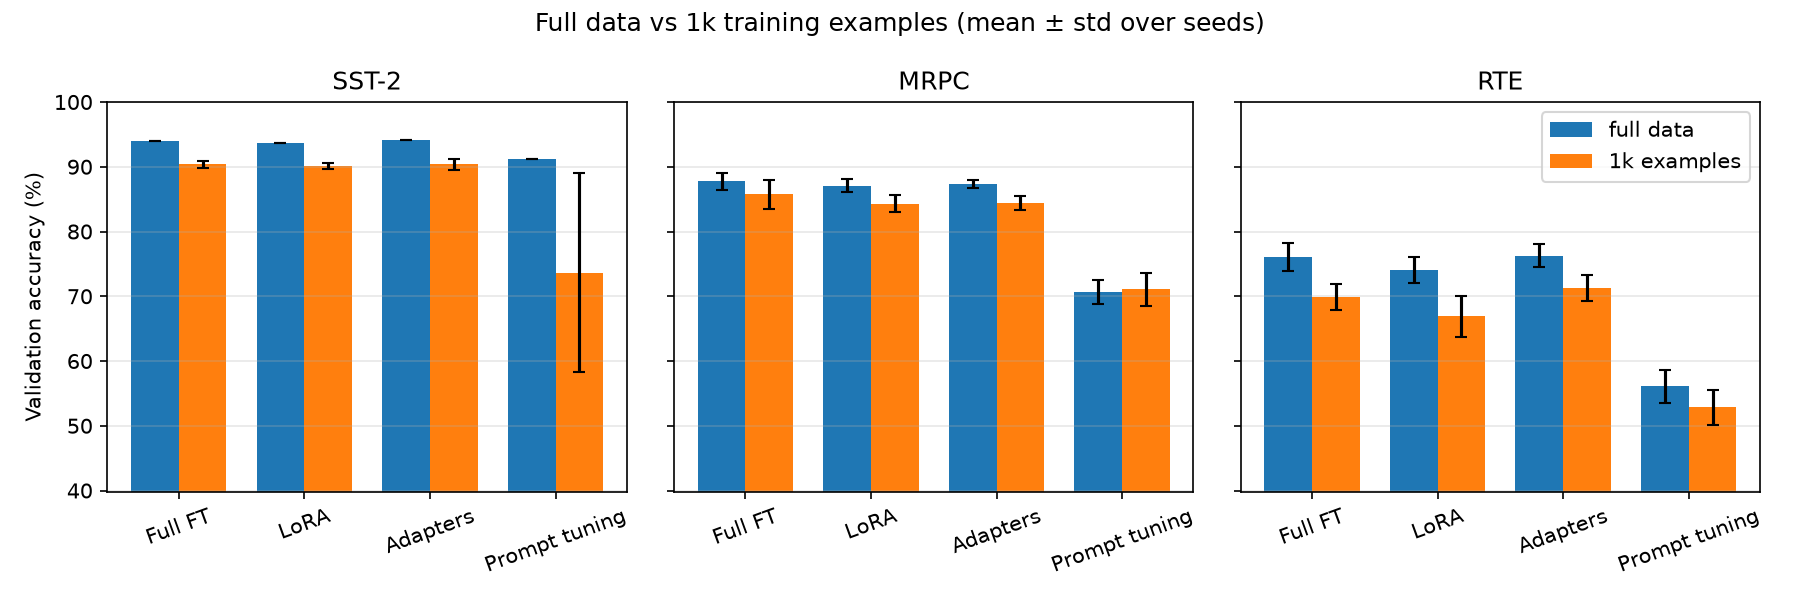
\includegraphics[width=0.9\textwidth]{figures/full_vs_1k.png}
  \caption{Validation accuracy with full training data vs 1,000 examples, per method and task.}
  \label{fig:lowdata}
\end{figure}

\subsection{Ablations}

Each ablation changes one setting of one method, on RTE with full data and seeds 1--3 (Table~\ref{tab:ablation}, Figure~\ref{fig:ablation}). The default row is the final run, and the learning rate is unchanged.

\begin{table}
  \caption{Ablations on RTE (full data), validation accuracy $\times$100, mean $\pm$ std over 3 seeds. ``Frozen $k$'' = embeddings and the bottom $k$ layers frozen; rf = reduction factor; * = default (final run). LoRA keeps $\alpha{=}2r$}
  \label{tab:ablation}
  \begin{minipage}{\textwidth}\footnotesize
    \begin{tabular}{llrrrr}
    \hline\hline
    Method & Setting & RTE acc & Params & Mem (MiB) & Time (s) \\
    \hline
    Full FT & frozen 0* & 76.1 $\pm$ 2.2 & 124.6M & 3,264 & 158 \\
     & frozen 3 & 75.2 $\pm$ 0.8 & 64.4M & 2,349 & 116 \\
     & frozen 6 & 73.0 $\pm$ 1.8 & 43.1M & 1,754 & 95 \\
     & frozen 9 & 65.3 $\pm$ 1.7 & 21.9M & 1,158 & 73 \\
    \hline
    LoRA & $r{=}1$ & 70.0 $\pm$ 1.4 & 0.63M & 1,932 & 109 \\
     & $r{=}4$ & 72.0 $\pm$ 3.7 & 0.74M & 1,934 & 110 \\
     & $r{=}8$* & 74.0 $\pm$ 2.0 & 0.89M & 1,937 & 112 \\
     & $r{=}16$ & 74.4 $\pm$ 0.0 & 1.18M & 1,943 & 110 \\
     & $r{=}64$ & 60.0 $\pm$ 10.3 & 2.95M & 1,975 & 110 \\
    \hline
    Adapters & Houlsby, rf 8 & 77.6 $\pm$ 1.9 & 4.15M & 1,926 & 107 \\
     & Houlsby, rf 16* & 76.3 $\pm$ 1.8 & 2.38M & 1,884 & 106 \\
     & Houlsby, rf 64 & 70.2 $\pm$ 2.9 & 1.05M & 1,853 & 105 \\
     & Pfeiffer, rf 16 & 74.1 $\pm$ 3.6 & 1.49M & 1,880 & 104 \\
    \hline
    Prompt & 5 tokens & 52.3 $\pm$ 2.5 & 0.60M & 1,796 & 105 \\
     & 20 tokens* & 56.1 $\pm$ 2.6 & 0.61M & 1,923 & 117 \\
     & 50 tokens & 53.2 $\pm$ 4.2 & 0.63M & 2,180 & 135 \\
     & 100 tokens & 52.6 $\pm$ 1.6 & 0.67M & 2,626 & 175 \\
     & 20 tokens, text init & 53.8 $\pm$ 1.6 & 0.61M & 1,923 & 111 \\
    \hline\hline
    \end{tabular}
  \end{minipage}
\end{table}

\paragraph{Partial Full FT is a poor alternative to PEFT.} Freezing the bottom 9 layers still trains 21.9M parameters but drops RTE accuracy to 65.3\%. LoRA trains 25 times fewer parameters and reaches 74.0\%. Freezing 3 layers keeps most of the accuracy (75.2\%) with 28\% less memory than Full FT, but it still uses more memory than any PEFT method.

\paragraph{LoRA rank.} Accuracy rises from $r{=}1$ (70.0) to $r{=}8$--16 (74.0--74.4) and collapses at $r{=}64$. There, two of three seeds stayed at majority-class level (52.7\% and 55.6\%), while the third reached 71.8\%. With $\alpha{=}2r$, a learning rate of 5e-4 appears too high for $r{=}64$. We did not re-tune it per rank, so this result shows instability at a fixed learning rate. It does not show that high ranks are worse in general.

\paragraph{Adapter size and type.} A larger bottleneck helps: reduction factor 8 reaches 77.6\%, the best RTE score in the study, with 4.2M trainable parameters and almost no extra memory. Reduction factor 64 loses 6 points. At the same reduction factor, the Pfeiffer configuration is 2.2 points below Houlsby, with 38\% fewer trainable parameters.

\paragraph{Prompt length and initialisation.} No setting moves prompt tuning more than 3.4 points above the majority class. Longer prompts make every input longer, so memory and time grow with prompt length (100 tokens: 2,626\,MiB and 175\,s) without any gain in accuracy. Initialising the prompt from a short text did not help either (53.8 vs 56.1).

\begin{figure}
  \centering
  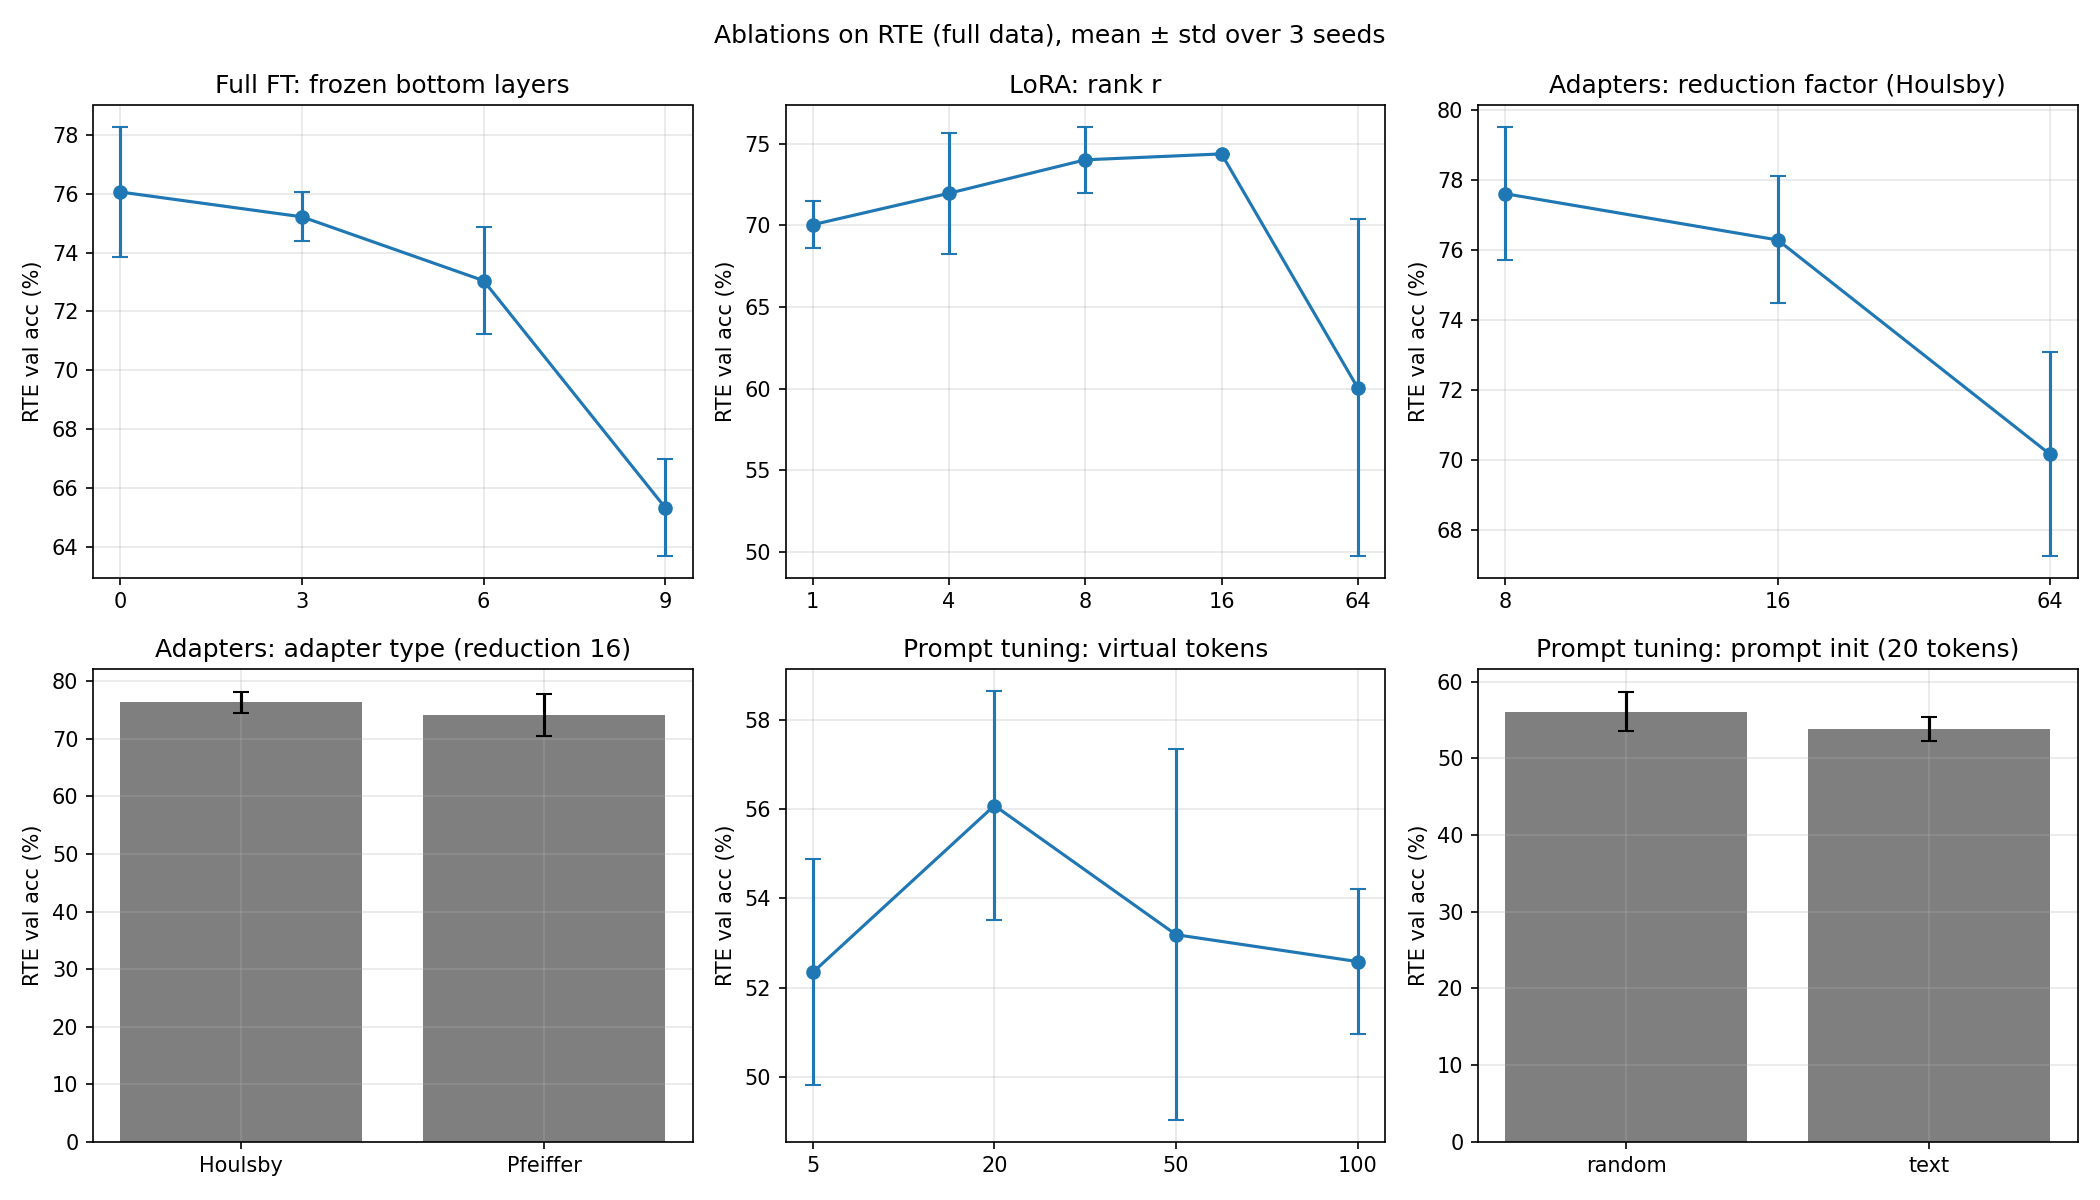
\includegraphics[width=\textwidth]{figures/ablations.png}
  \caption{Ablations on RTE (full data), mean $\pm$ std over 3 seeds.}
  \label{fig:ablation}
\end{figure}

\section{Discussion}

\paragraph{Why prompt tuning is weak on \texttt{roberta-base}.} Prompt tuning trains only 15,360 prompt parameters and changes the model's behaviour only through attention to those 20 positions. Lester {\it et al.} \shortcite{lester2021} found that this works only when the frozen model is very large: for T5, prompt tuning matched full fine-tuning only at about 11B parameters. \texttt{roberta-base} has 125M parameters, so our results agree with that finding. The ablations show that the problem is not the prompt length or the initialisation. Prompt tuning did learn SST-2 with 67k examples. At this scale and budget it could not learn two tasks: sentence-pair inference with 2.5k examples (RTE) and paraphrase detection with 3.7k examples (MRPC).

\paragraph{Why adapters can match Full FT.} RTE and MRPC have only a few thousand training examples, and Full FT overfits easily on them (RTE dev accuracy varies by $\pm$4.4 points across seeds). Adapters keep the pretrained weights fixed and add a small change to each layer, which limits how far the model can move from its pretrained state. The ablations show that capacity still matters: reduction factor 8 helped and 64 hurt.

\paragraph{Recommendations.}
\begin{itemize}
  \item {\it Limited GPU memory:} adapters or LoRA. They peak at about 1.9\,GB vs 3.3\,GB for Full FT and lose at most 2.1 points.
  \item {\it Limited training time:} LoRA on large datasets (324 vs 492\,s on SST-2), adapters on small ones (106 vs 158\,s on RTE).
  \item {\it Very little data:} adapters or Full FT, which lose the least with 1k examples. Avoid prompt tuning, which is unstable.
  \item {\it Many tasks served from one model:} LoRA. It needs 3.4\,MB per task, and the update can be merged into the weights, so inference costs nothing extra.
\end{itemize}

\section{Conclusion}

With one shared budget on \texttt{roberta-base}, adapters and LoRA keep almost all of Full FT's accuracy on SST-2, MRPC and RTE. They train 0.7--1.9\% of the parameters, use about 40\% less GPU memory and need 3--9\,MB per task instead of 475\,MB. With 1,000 training examples, Full FT and adapters lose the least accuracy. Prompt tuning has the smallest checkpoint, but at this model size it stays near the majority-class baseline on MRPC and RTE and is unstable with little data. Freezing layers of Full FT is a much worse trade-off than either LoRA or adapters.

\section{Limitations}

\begin{itemize}
  \item SST-2 full data has only one seed per method, so the SST-2 full numbers have no standard deviation and should not be read as a ranking.
  \item Three seeds are few for RTE and MRPC, and many of our differences are smaller than one standard deviation.
  \item The LR search was run after the final runs, with seed 1 only.
  \item The ablations are on RTE only, and the learning rate was not re-tuned for each setting. This matters most for LoRA $r{=}64$.
  \item All methods get the same number of epochs, but prompt tuning was often still improving at the last epoch.
  \item The 10\% dev split is drawn with the run's seed, so dev accuracy varies more than validation accuracy.
  \item Peak memory is \texttt{max\_memory\_allocated}, which leaves out the allocator cache.
  \item Adapters use AdapterHub instead of Hugging Face PEFT, because PEFT has no Houlsby adapters.
  \item We report on the GLUE validation split because test labels are hidden. The validation split was never used for any choice.
\end{itemize}

\section*{Team contributions}

Deepak Mandal: full fine-tuning (16 runs), repository, data pipeline, training and Kaggle run scripts. Anoop Kumar: LoRA (16 runs), results format and validation, analysis notebook, LR search and ablation runs. Chiranjeet Biswas: adapters (16 runs), background and literature review. Byagari Praveen Kumar: prompt tuning (16 runs), results tables, plots and slides.

\begin{thebibliography}{}
  \bibitem[\protect\citename{Houlsby {\it et al.}\ }2019]{houlsby2019}
   Houlsby, N., Giurgiu, A., Jastrzebski, S., Morrone, B., de Laroussilhe, Q.,
   Gesmundo, A., Attariyan, M. and Gelly, S. (2019) Parameter-efficient transfer
   learning for NLP. In {\it Proceedings of the 36th International Conference on
   Machine Learning (ICML)}. \url{https://arxiv.org/abs/1902.00751}
  \bibitem[\protect\citename{Hu {\it et al.}\ }2022]{hu2022}
   Hu, E. J., Shen, Y., Wallis, P., Allen-Zhu, Z., Li, Y., Wang, S., Wang, L.
   and Chen, W. (2022) LoRA: low-rank adaptation of large language models. In
   {\it International Conference on Learning Representations (ICLR)}.
   \url{https://arxiv.org/abs/2106.09685}
  \bibitem[\protect\citename{Lester {\it et al.}\ }2021]{lester2021}
   Lester, B., Al-Rfou, R. and Constant, N. (2021) The power of scale for
   parameter-efficient prompt tuning. In {\it Proceedings of the 2021 Conference
   on Empirical Methods in Natural Language Processing (EMNLP)}.
   \url{https://arxiv.org/abs/2104.08691}
  \bibitem[\protect\citename{Liu {\it et al.}\ }2019]{liu2019}
   Liu, Y., Ott, M., Goyal, N., Du, J., Joshi, M., Chen, D., Levy, O., Lewis, M.,
   Zettlemoyer, L. and Stoyanov, V. (2019) RoBERTa: a robustly optimized BERT
   pretraining approach. {\it arXiv preprint} arXiv:1907.11692.
  \bibitem[\protect\citename{Pfeiffer {\it et al.}\ }2021]{pfeiffer2021}
   Pfeiffer, J., Kamath, A., R\"uckl\'e, A., Cho, K. and Gurevych, I. (2021)
   AdapterFusion: non-destructive task composition for transfer learning. In
   {\it Proceedings of the 16th Conference of the European Chapter of the
   Association for Computational Linguistics (EACL)}.
   \url{https://arxiv.org/abs/2005.00247}
  \bibitem[\protect\citename{Wang {\it et al.}\ }2019]{wang2019}
   Wang, A., Singh, A., Michael, J., Hill, F., Levy, O. and Bowman, S. R. (2019)
   GLUE: a multi-task benchmark and analysis platform for natural language
   understanding. In {\it International Conference on Learning Representations
   (ICLR)}. \url{https://arxiv.org/abs/1804.07461}
\end{thebibliography}

\label{lastpage}

\end{document}
